\pagebreak
\subsection{Generator Constant}%\label{generatorConstant}
\textbf{Name: Group 510}\\
\textbf{Date: 30/09 - 2015}

\subsubsection{Purpose}
The purpose of the test is to find the generator constant $K_e$ by measuring the motor voltages, currents and velocities, in several steady states.

\subsubsection{Setup}
\begin{figure}[H]
  \centering
	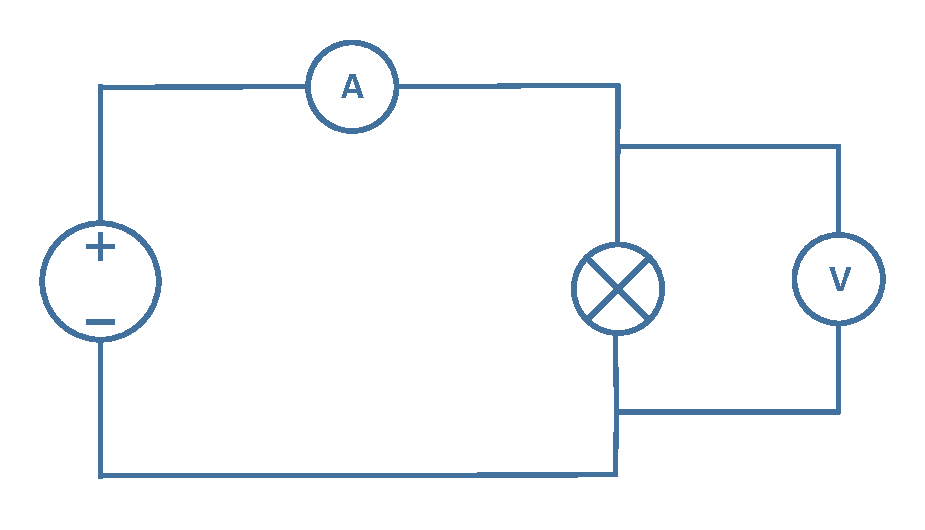
\includegraphics[scale=0.5]{figures/MotorTest4.pdf}
	\caption{Setup diagram}
\end{figure}

\subsubsection{List of Equipment}

\begin{table}[H]
\begin{tabular}{|l|l|p{4cm}|}
\hline%------------------------------------------------------------------------------------
  \textbf{Instrument}                        &  \textbf{AAU-no.}  &  \textbf{Type}       \\
\hline%------------------------------------------------------------------------------------
  Multimeter 1                               &  60764             &  Fluke 189 True RMS  \\
\hline%------------------------------------------------------------------------------------
  Multimeter 2                   		         &  60769             &  Fluke 189 True RMS  \\
\hline%------------------------------------------------------------------------------------
  Power Supply ($0 - 32$ V) ($0 - 10$ A)     &  77076             &  Ea - ps 7032 - 100  \\
\hline%------------------------------------------------------------------------------------
  Optical tachometer                         &  08246             &  Shimpo DT-205       \\
\hline%------------------------------------------------------------------------------------
\end{tabular}
\end{table}

\subsubsection{Procedure}

\begin{enumerate}
  \item Turn on the two multimeters and put them in ampere and voltage mode respectively.
  \item Apply $1$ V by use of the voltage mode multimeter
  \item Read out the current value from the ampere mode multimeter
  \item Read out RPM of the motor using the optical tachometer.
  \item Repeat the past $3$ steps up to $7$ V in $1$ V increments.
\end{enumerate}

\subsubsection{Results}

\begin{table}[H]
\begin{tabular}{|l|l|l|l|}
\hline%---------------------------------------------------------------------------------------------
  \textbf{Input (V)}  & \textbf{Output (A)} & \textbf{Output (RPM)} & \textbf{Generator constant} \\
\hline%---------------------------------------------------------------------------------------------
  $1$                 &            $1.7$    &  $3684$               & $0.00181$                   \\
\hline%---------------------------------------------------------------------------------------------
  $2$                 &            $2.2$    &  $8063$               & $0.00191$                   \\
\hline%---------------------------------------------------------------------------------------------
  $3$                 &            $2.6$    &  $12021$              & $0.00202$                   \\
\hline%---------------------------------------------------------------------------------------------
  $4$                 &            $3.3$    &  $16746$              & $0.00195$                   \\
\hline%---------------------------------------------------------------------------------------------
  $5$                 &            $4.1$    &  $21966$              & $0.00186$                   \\
\hline%---------------------------------------------------------------------------------------------
  $6$                 &            $4.8$    &  $26420$              & $0.00186$                   \\
\hline%---------------------------------------------------------------------------------------------
  $7$                 &            $5.6$    &  $31447$              & $0.00182$                   \\
\hline%---------------------------------------------------------------------------------------------
\end{tabular}
\end{table}
%
The equation for the generator constant is given by:
\begin{flalign}
  K_e = \frac{U_a - R_a I_a}{\omega} \unit{Wb}\nonumber
\end{flalign}
\hspace{6mm} Where:\\
\begin{tabular}{p{1cm}ll}
  & $\omega$ & is the angular velocity in rad/s \\
  & $R_a$    & is the armature resistance       \\
  & $I_a$    & is the armature current          \\
  & $K_e$    & is the generator constant        \\
\end{tabular}

The generator constants for each measurement is not equal, but with a small margin in difference. The average generator constant is:
\begin{flalign}
  K_e = 0.00189 \unit{Wb}\nonumber
\end{flalign}